\documentclass[oneside,a4paper,11pt,explicit]{book}
\usepackage[utf8]{inputenc}
\usepackage[sedes]{kultem}
\usepackage[english]{babel}
% \usepackage[dutch]{babel}

%% INSERT YOUR PACKAGES HERE
\usepackage[accsupp]{axessibility}  % improves PDF readability for those with disabilities.
\usepackage[hidelinks]{hyperref}
\usepackage{lipsum}
\usepackage{listings}

%% TITLE PAGE OPTIONS (only works with \maketitle is called in the document)
\title{Judul Buku}
\subtitle{Template Buku di Penerbit Jala Marwita Lestari}
\date{\today}
\author{Bambang Purnomosidi D. P.}
%\professor{We Don't Know (yet)}

%% DOCUMENT
\begin{document}
\maketitle

\chapter{Example}
\kulbox{{\bf Note:} This is a nice box where you can put a lot of information concerning the following chapter. How much pages are required for an assignment for example, or an important change of notation.}
\lipsum[1]

\section{Some questions}
\lipsum[2]

As an example, we will consider the equation of the Duffing oscillator
\begin{equation}
\ddot{x}+k\dot{x}+x^3=B\cos t,
\end{equation}
with $k=0.1$ and $B=11$ and answer the following questions

\begin{questions}
\question Can you show that the model exhibits a chaotic regime?
\begin{tasks}
\task By performing a qualitative analysis of a simulation?
\task By computing the Lyapunov exponents of the system?
\end{tasks}
\question What is the dimension of the system?
\question Simulate the model for another choice of parameters. What do you observe?
\end{questions}

\section{A Wild Figure Appears!}
\lipsum[3] This can be seen at figure~\ref{fig:example}.

\begin{figure}[h]
    \centering
    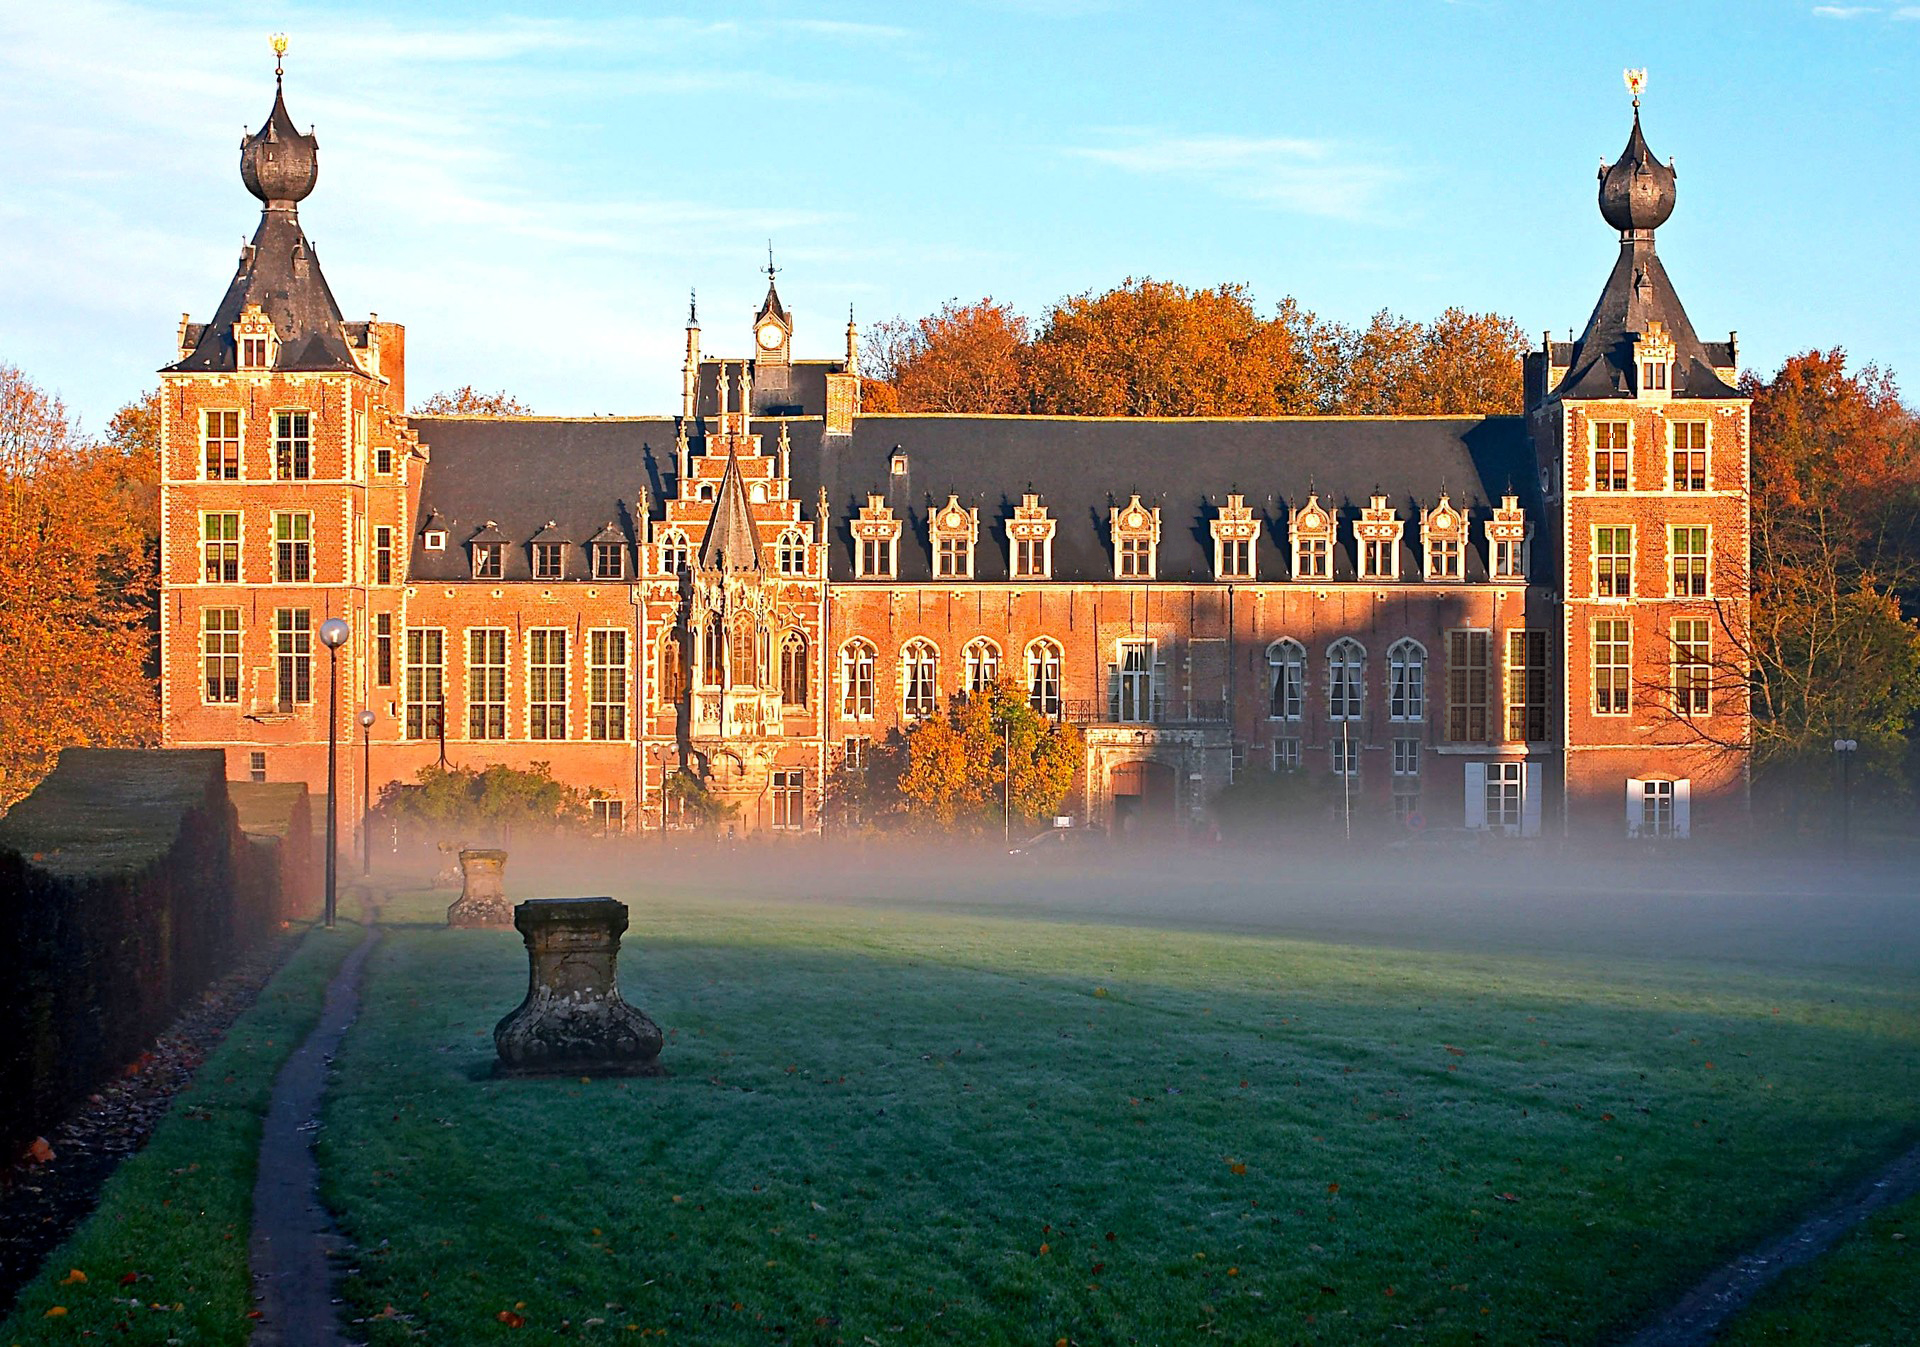
\includegraphics[width=\textwidth]{img/arenberg.jpg}
    \caption{The castle of Arenberg in Heverlee, with windows corrected.}
    \label{fig:example}
\end{figure}

\chapter{Short Manual}
\lstset{basicstyle=\ttfamily,breaklines=true}
We now present some commands that you can use. If you experience any bugs, don't hesitate to report them on the corresponding repository: \url{https://github.com/hdeplaen/kultem}. If you can fix the bug or just want to improve the work and add a new functionality, don't hesitate to contribute with a push request.
\section{Package}
To use the package, it suffices to include \verb|\usepackage[<options>]{kultem}|. The package admits the following option
\begin{itemize}
    \item \verb|sedes|: prints the \emph{Sedes Sapientiae} of the university as watermark on the title page.
\end{itemize}

\section{Title Page}
The available title options are (from top to bottom):
\begin{itemize}
    \item \verb|\title{<text>}|: the title of the document;
    \item \verb|\subtitle{<text>}|: the subtitle of the document (may be omited);
    \item \verb|\author{<text>}|: the author of the document;
    \item \verb|\promoter{<text>}|: the promoter (singular);
    \item \verb|\promoters{<text>}|: the promoters (plural, seperate the names with a comma or a \verb|\\| if you want them to be written on different lines);
    \item \verb|supercom{<text>}|: supervisory commitee  (singular and plural undifferentiated);
    \item \verb|jury{<text>}|: jury (singular and plural undifferentiated);
    \item \verb|assessors{<text>}|: assessors (plural, we did not consider the singular option);
    \item \verb|professor{<text>}|:  professor (singular);
    \item \verb|professors{<text>}|: professors (plural, seperate the names with a comma or a \verb|\\| if you want them to be written on different lines); 
    \item \verb|assistant{<text>}|: assistant (singular);
    \item \verb|assistants{<text>}|: assistants (seperate the names with a comma or a \verb|\\| if you want them to be written on different lines);
    \item \verb|\date{<text>}|: the date (one may consider the command \verb|\today| for an automatic filling).
    \item \verb|\coverimage{<path_to_image>}|: this prints an image on the cover (to avoid a heavy looking title page, we do not recommend to combine it with the package option \verb|sedes| or the command \verb|\coversvg| and \verb|coverinput|);
    \item \verb|\coversvg{<path_to_svg>}|: similar to the previous option, but prints an svg on the cover instead of an image (to avoid a heavy looking title page, we do not recommend to combine it with the package option \verb|sedes| or the command \verb|\coverimage| and \verb|coverinput|);
    \item \verb|\converinput{<path_to_file>}|: similar to the previous option, but allows to directly input a block of code instead of an image, \emph{e.g.} a TikZ picture (to avoid a heavy looking title page, we do not recommend to combine it with the package option \verb|sedes| or the command \verb|\coverimage| and \verb|\coversvg|).
\end{itemize}

\section{Questions and Tasks}
These are two variants of the \verb|enumerate| environment. The can be called apart from each other as in what follows or nested like in the beginning example.
\begin{lstlisting}
\begin{questions}
    \item What is on your bucket list?
    \item What are you most thankful for?
    \item What are you most afraid of?
    \item What are you most passionate about?
\end{questions}
\end{lstlisting}
\begin{questions}
    \item What is on your bucket list?
    \item What are you most thankful for?
    \item What are you most afraid of?
    \item What are you most passionate about?
\end{questions}

\begin{lstlisting}
\begin{tasks}
    \item Correct the \verb|bindingoffset| option;
    \item Implement an image command for the title page.
\end{tasks}
\end{lstlisting}
\begin{tasks}
    \item Correct the \verb|bindingoffset| option;
    \item Implement an image command for the title page.
\end{tasks}

\section{kulbox}
The \verb|kulbox[<margin>]{<text>}| command allows you to create a nice blue box containing some text. The default margin is equal to 3pt and we do not advise on changing it and just omit it to use the default value:
\begin{lstlisting}
    \kulbox{This is a nice kulbox omiting the margin option.}
\end{lstlisting}
\kulbox{This is a nice kulbox omiting the margin option.}

In case you would however really want to change it, you can specify your custom margin:
\begin{lstlisting}
    \kulbox[0pt]{This is an ugly cramped kulbox with no margin.}
\end{lstlisting}
\kulbox[0pt]{This is an ugly cramped kulbox with no margin.}
\begin{lstlisting}
    \kulbox[10pt]{This is an extravagant bulky kulbox with a huge margin.}
\end{lstlisting}
\kulbox[10pt]{This is an extravagant bulky kulbox with a huge margin.}

\section{bindingoffset}
This adds a default binding offset as in the \verb|geometry| package, with a fixed value of 12mm. You can call it with \verb|\usepackage[bindingoffset]{kultem}|. \textbf{Warning:} the headers are for the moment not compatible with this option and will remain unchanged.

\end{document}
